\clearpage
\section{Standalone MISO square-wave test: 15 November 2026}
A temporary image (\texttt{399ead20}) adds a runtime MISO generator. It retains
LVCMOS33 DRIVE12/SLEW SLOW and uses the original DD29/47-ohm/cable path.
Nonzero generator modes continuously enable the FPGA output, overriding
HSEL-controlled tri-state. The modes select static low, static high or a square
wave. The original SPI parser is held deselected during these comparisons;
Kasli SEL/SCK/MOSI remain actively driven at idle. No external transmitter
is attached to the MISO net, and no buffer direction or external PLL setting changes.

The divider runs from MCLK1 at nominal 40.0787 MHz, with 20039 ticks per half
period, producing 1000.017466 Hz. Mode registers and generator state are
independent of SYS reset. Two synchronizer stages cross the mode control.
Simulation verified static modes, normal-mode return and half-period spacing.
Dell timing qualification passed with setup slack 0.084 ns and hold slack 0.060 ns.

\begin{center}\begin{tabular}{lrrr}\toprule
Condition & Windows & SYS reset/LOCK loss & MISO edges\\\midrule
Normal SPI before &6&6/6&88\\
Static low, first block &6&0/6&0\\
1 kHz, first block &12&0/12&6108\\
Static high &6&0/6&0\\
1 kHz, second block &12&0/12&6108\\
Static low, return &6&0/6&0\\
Normal SPI after &6&6/6&96\\\bottomrule
\end{tabular}\end{center}
All normal SPI signatures were correct. Independent raw validation confirms
no sampled activity on SEL, SCK or MOSI during generator windows, the parser
hold state, disabled explicit clamp, and the retained generator mode.

The standalone waveform did not reproduce the failure: 12216 sampled MISO
transitions across 24 windows, with no observed SYS reset or LOCK loss.
Static low/high comparisons were also quiet. Normal SPI positive controls
reproduced before and after. Thus continuously driven 1 kHz MISO activity
alone is insufficient under this test. It does not rule out interference
sensitive to SPI edge timing, phase, bit patterns, simultaneous lines or
HSEL-controlled output-enable transitions. The pulse test deliberately
keeps MISO enabled, unlike normal SPI idle.

The generator and observer share the clock-chip-derived MCLK1 reference;
a complete common reference stop is not observable with this setup.
The recorded signal is the logical MISO source, not pad voltage or an
oscilloscope measurement of clock integrity. Static windows stop after about
one nominal second; pulse windows usually fill the 512-record buffer in about
0.255 nominal seconds. Sparse last-event timestamps do not measure the full
static exposure duration.

\begin{center}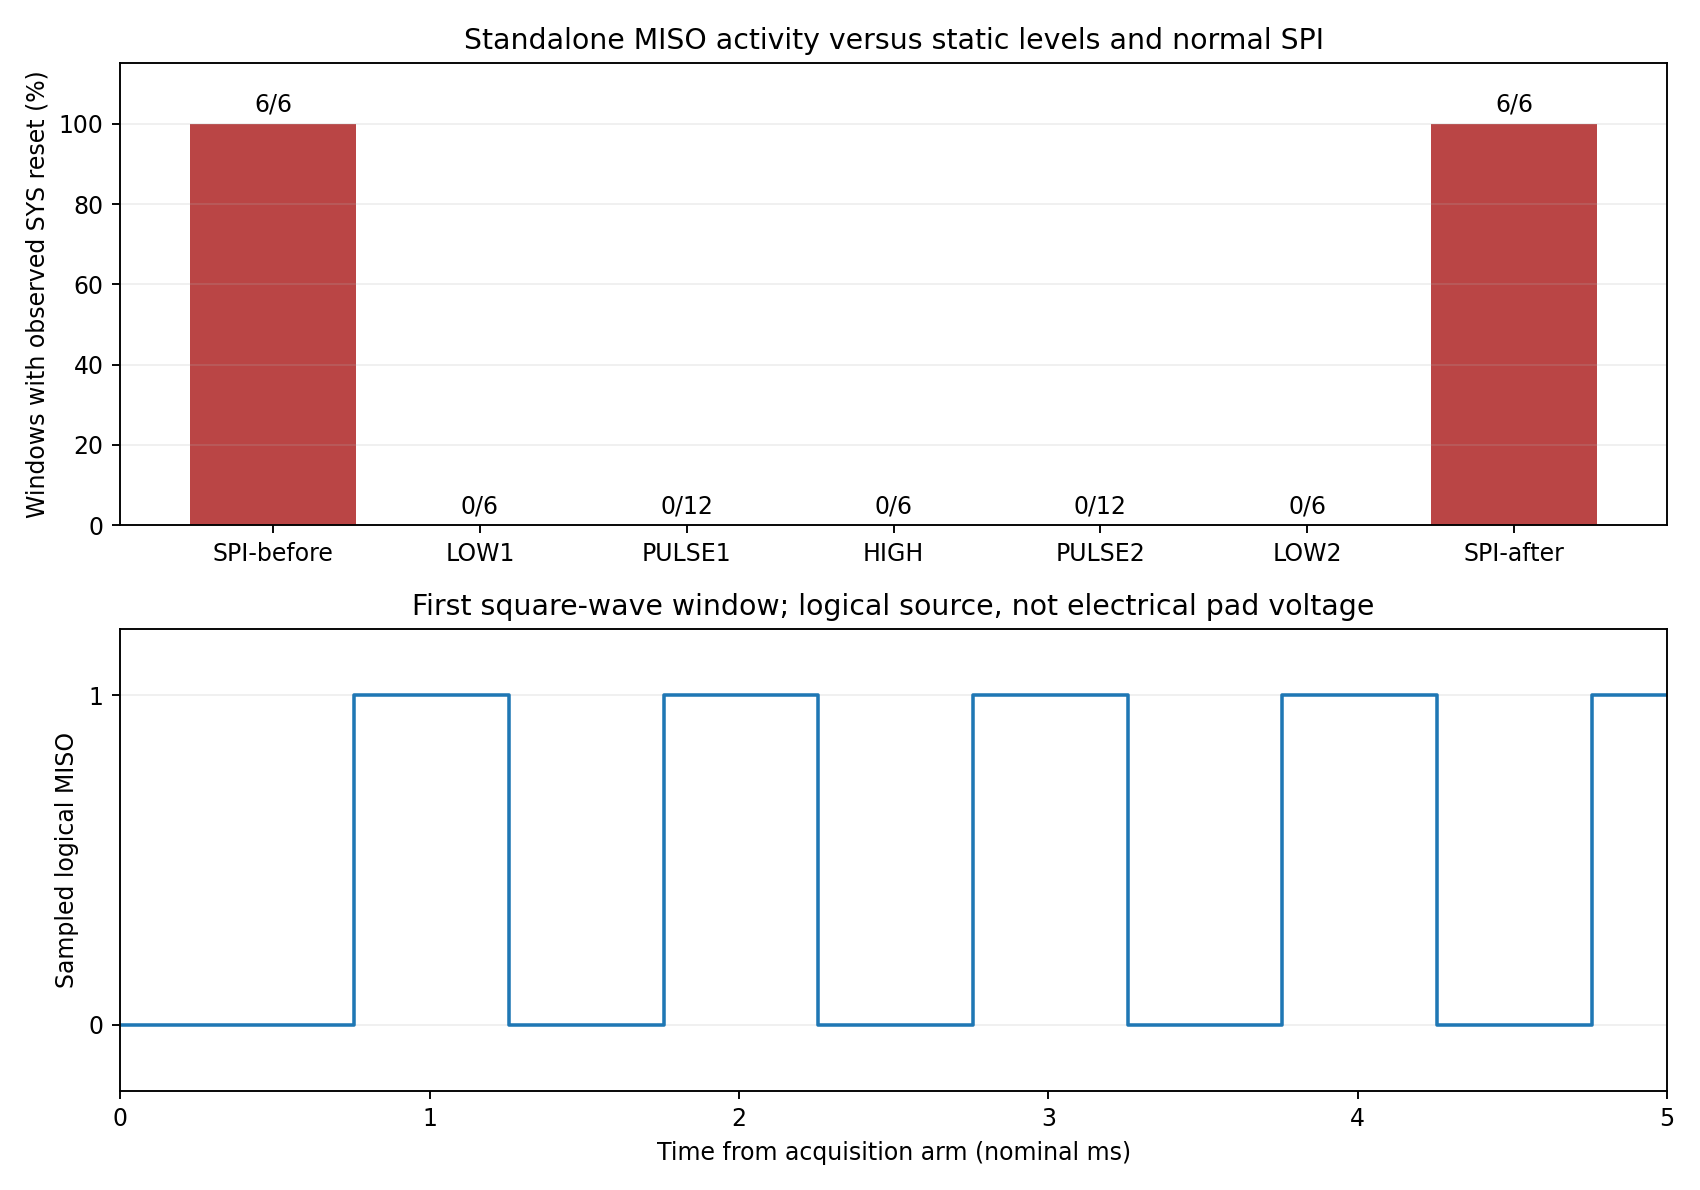
\includegraphics[width=\linewidth]{miso-generator.png}\end{center}
Raw captures, source/bitstream, simulation and load/restore receipts are retained
in the evidence directory:
\begin{center}\path{system/evidence-miso-generator-20261115}\end{center}

Exact original c7531465 was restored successfully. Final frontend readiness
was 0xfff, power-good was healthy, and all twelve physical ADC bank-A captures
passed on the first attempt. All hardware leases were released.
